% El avance de las tecnologías de la información ha permitido el desarrollo de sofisticadas herramientas de visualización y análisis de datos, fundamentales para la toma de decisiones en entornos empresariales dinámicos. En el contexto de la CVC y la sostenibilidad, estas herramientas facilitan la interpretación de grandes volúmenes de datos y el monitoreo en tiempo real de indicadores estratégicos, siendo factotes cruciales para que las Pymes puedan competir en mercados cada vez más digitales. Entre las principales herramientas utilizadas se destacan:


% \begin{itemize}
%     \item \textbf{Plataformas de Dashboards Interactivos:}  
%     \emph{Power BI} y \emph{Tableau} son dos de las plataformas líderes en la creación de tableros interactivos. Estas herramientas permiten integrar datos provenientes de múltiples fuentes, aplicar filtros dinámicos y presentar la información de manera gráfica, facilitando la identificación de tendencias y patrones relevantes. Microsoft, por ejemplo, ha destacado en su noticia “Microsoft dota de inteligencia de datos a las empresas pequeñas con Power BI” cómo esta plataforma democratiza el acceso a análisis avanzados, permitiendo a las Pymes transformar grandes volúmenes de datos en información estratégica para la toma de decisiones \cite{PowerBI_News2023}.
    
%     \item \textbf{Librerías de Visualización en Python:}  
%     Herramientas como \emph{Plotly}, \emph{Dash} y \emph{Seaborn} ofrecen una gran flexibilidad para desarrollar soluciones personalizadas de visualización. Estas librerías permiten crear gráficos interactivos, heatmaps y dashboards que se integran en aplicaciones web, facilitando el acceso a la información en tiempo real y adaptándose a las necesidades específicas de los modelos predictivos.
    
%     \item \textbf{Sistemas de Integración y Consolidación de Datos:}  
%     La efectividad de las herramientas de visualización depende en gran medida de la capacidad para integrar y consolidar datos de diversas fuentes. Herramientas ETL (Extract, Transform, Load) y bases de datos de alto rendimiento permiten centralizar la información, garantizando que los datos presentados sean consistentes y actualizados.
% \end{itemize}

% El uso combinado de estas tecnologías no solo permite visualizar el output de los modelos predictivos, sino que también posibilita la generación de informes personalizados y el monitoreo de indicadores clave (KPIs) relacionados con la CVC y la sostenibilidad. La Figura~\ref{fig:Dashboard_Ejemplo} muestra un ejemplo de un tablero interactivo desarrollado en Power BI por Microsoft para monitorear estos indicadores en tiempo real, facilitando la toma de decisiones estratégicas en Pymes \cite{PowerBI_News2023}.

% \begin{figure}[h!]
%   \centering
%   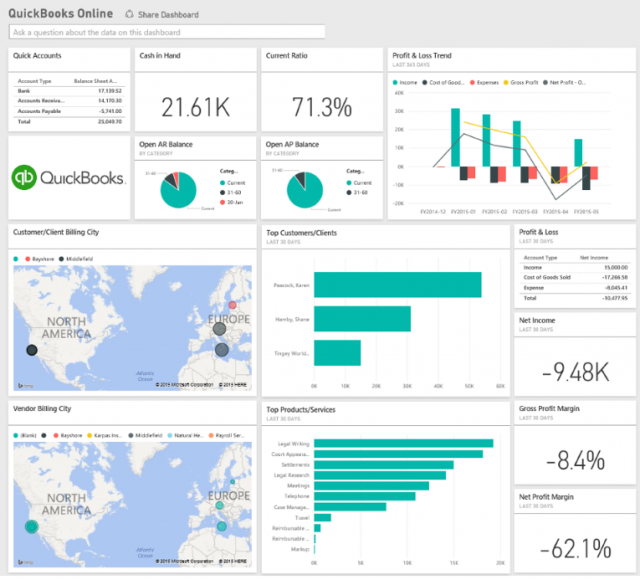
\includegraphics[width=0.75\textwidth]{images/Power-BI_QBO_Pymespng.png}
%   \caption{Ejemplo de tablero interactivo para la visualización de indicadores estratégicos en Pymes.}
%   \label{fig:Dashboard_Ejemplo}
% \end{figure}







% % % ====================== OPC UA ======================
% % Los protocolos de comunicación forman parte de nuestra investigación, para el entendimiento de las comunicaciones que se presentan en la funcionalidad de la celda de Manufactura Flexible del CAP. Esto con el fin de conocer su funcionamiento a profundidad y de los protocolos y normas existentes detrás de estas comunicaciones.\newline

% % \subsection{OPC UA (Arquitectura Unificada de Comunicaciones de Plataforma
% % Abierta)}
% % Es una arquitectura orientada a servicios independiente de la plataforma que integra toda la funcionalidad de las especificaciones individuales de OPC Classic en un marco extensible que proporciona soluciones más robustas, seguras y escalables para la comunicación industrial \cite{OPC_Foundation_2019_UA} \cite{OPC_Foundation_2020_Classic}. \\

% % A diferencia de OPC Classic, OPC UA puede funcionar en diferentes sistemas operativos, como Windows, Linux y otros. Utiliza protocolos estándar de Internet, como TCP/IP y HTTPS, para la comunicación, lo que facilita la interoperabilidad entre dispositivos y aplicaciones en entornos heterogéneos. Una de las principales ventajas de OPC UA es su enfoque en la seguridad. Proporciona mecanismos de autenticación, autorización y cifrado de extremo a extremo para proteger la comunicación y los datos transmitidos. Además, ofrece características avanzadas, como un modelo de información flexible, soporte para datos históricos, notificación de eventos y gestión de alarmas \cite{OPC_Foundation_2019_UA} \cite{paessler} \cite{siemens_ag_2017}. \\

% % OPC-UA se ha convertido en el estándar de facto para la comunicación industrial y ha sido adoptado por muchas empresas y organizaciones en todo el mundo. La norma \textbf{IEC 62541} define las especificaciones técnicas para la implementación de OPC UA, brindando un marco común y coherente para su implementación y uso en diversos sectores de la industria \cite{Person_ICONICS_INC_2008} \cite{INTERNATIONAL_ELECTROTECHNICAL_COMMISSION_2020}.\\

% % Las principales especificaciones técnicas definidas por la norma \textbf{IEC 62541} son las siguientes:

% % \begin{enumerate}
% %   \item \textbf{Modelo de información:} Se establecen las estructuras de datos y la semántica utilizada para describir la información intercambiada entre los sistemas a través de OPC UA. Esto incluye la definición de nodos, atributos, métodos y eventos.
% %   \item \textbf{Protocolo de comunicación:} Se especifica el protocolo de comunicación utilizado para la transferencia de datos entre los sistemas. OPC UA utiliza un modelo cliente-servidor, donde los clientes solicitan y reciben datos de los servidores. El protocolo puede basarse en TCP/IP y soportar diferentes mecanismos de transporte y seguridad.
% %   \item \textbf{Seguridad:} Se definen los mecanismos de seguridad utilizados para proteger la comunicación y los datos transmitidos en OPC UA. Esto incluye autenticación, autorización, cifrado y firma digital, entre otros aspectos.
% %   \item \textbf{Descubrimiento y conexión:} Se describe cómo los clientes pueden descubrir y conectarse a los servidores OPC UA disponibles en la red. Esto puede implicar la resolución de nombres, la búsqueda de servicios de directorio y la negociación de las opciones de comunicación.
% %   \item \textbf{Historial de datos:} Se establece cómo se almacenan y acceden a los datos históricos en OPC UA. Esto puede incluir la capacidad de almacenamiento local en los servidores y la consulta de datos históricos por parte de los clientes.
% %   \item \textbf{Alarmas y eventos:} Se establece el mecanismo para el manejo de alarmas y eventos en OPC UA. Permite a los servidores notificar a los clientes sobre cambios de estado, condiciones de error o eventos relevantes.

% % \end{enumerate}

% % % ====================== Ethernet % ======================
% % \subsection{Ethernet Industrial}
% % Es el uso de Ethernet en un entorno industrial con protocolos que proporcionan determinismo y control en tiempo real. Los protocolos para Ethernet industrial incluyen EtherCAT , EtherNet/IP , PROFINET , POWERLINK , SERCOS III , CC-Link IE y Modbus TCP \cite{Lin_Pearson_TexasInst_2018}. En el caso de la celda de manufactura del CAP, esta utiliza el protocolo de Modbus TCP (también Modbus TCP/IP), el cual es una extensión de Modbus RTU con una interfaz TCP que se ejecuta en Ethernet a través del puerto 502 y fue desarrollado originalmente por Schneider Electric. Además, Modbus es un bus serial sencillo, robusto y libre de derechos de autor que es fácil de implementar y funciona en enlaces físicos RS-232 o RS-485 con velocidades de hasta 115K baudios. \cite{ACROMAG_INCORPORATED_2005} \cite{ENCODER_PRODUCTS_COMPANY_2019}.\\

% % Por otro lado, Ethernet se está convirtiendo en omnipresente y rentable, con enlaces físicos comunes y mayor velocidad, por ello, muchos protocolos de comunicación industrial se están pasando a soluciones basadas en esta tecnología, permitiendo así una topología de red flexible y un número de nodos en el sistema \cite{Lin_Pearson_TexasInst_2018}.

% % % ====================== TCP/IP % ======================
% % \subsection{Modbus TCP/IP }
% % Fue desarrollado bajo la unión del protocolo de aplicación Modbus con la transmisión Ethernet \textbf{IEEE 802.3} tradicional. El Protocolo de control de transporte (TCP) reside una capa por encima del Protocolo de Internet (IP) y es responsable de transportar los datos de la aplicación y hacerlos seguros, mientras que IP es responsable del direccionamiento real y la entrega de los datos \cite{Andersdotter_Lansford_Law_Marks_Myles_2023}. \\

% % Por un lado, el paquete TCP se inserta en la porción de datos del paquete IP debajo de él, mientras que IP en sí mismo es un protocolo no seguro y sin conexión y debe funcionar junto con el TCP superpuesto para poder operar. De esta forma, TCP generalmente se considera la capa superior de la plataforma IP que sirve para garantizar la transferencia segura de datos \cite{ACROMAG_INCORPORATED_2005}. Para implementar una comunicación Modbus se deben tener en cuenta las siguientes reglas según la organización de Modbus \cite{Modbus_Organization_2006}:

% % \begin{enumerate}
% %     \item Sin requisitos explícitos del usuario, se recomienda implementar la gestión automática de conexiones TCP.
% %     \item Se recomienda mantener la conexión TCP abierta con un dispositivo remoto y no abrirla y cerrarla para cada transacción MODBUS/TCP. Observación: Sin embargo, el cliente MODBUS debe ser capaz de aceptar una solicitud de cierre del servidor y cerrar la conexión. . La conexión se puede reabrir cuando sea necesario.
% %     \item Se recomienda que un Cliente MODBUS abra un mínimo de conexiones TCP con un servidor MODBUS remoto (con la misma dirección IP). Una conexión por aplicación podría ser una buena opción.
% %     \item Se pueden activar varias transacciones MODBUS simultáneamente en la misma conexión TCP. Observación: si se hace esto, entonces se debe usar el identificador de transacción MODBUS para identificar de manera única las solicitudes y respuestas coincidentes.
% %     \item En el caso de una comunicación bidireccional entre dos entidades MODBUS remotas (cada una de ellas es cliente y servidor), es necesario abrir conexiones separadas para el flujo de datos del cliente y para el flujo de datos del servidor.
% %     \item Una trama/frame TCP debe transportar solo una ADU MODBUS. Se desaconseja enviar múltiples solicitudes o respuestas MODBUS en la misma PDU TCP.
% % \end{enumerate}

% % % ====================== Comunicación Serial RS232 y señales digitales I/O ======================
% % \subsection{Comunicación Serial RS232 y señales digitales I/O }
% % El protocolo de comunicación RS232 (Estándar Recomendado 232 por sus siglas en inglés) fue introducido por primera vez en 1960 por la Electronic Industries Association (EIA)   es uno de los más antiguos pero populares que se utiliza a nivel industrial. Este es un tipo de tipo de comunicación serial utilizada para la transmisión de datos normalmente en distancias medias \cite{Sharma_2018}. No obstante, el estándar ha cambiado de nombre varias veces durante su historia a medida que la organización cambió su nombre, y ha sido conocido como EIA RS-232, EIA 232 y, más recientemente, como TIA 232 desde 1988 por la Telecommunications Industry Association (TIA). \\

% % Debido a que RS-232 se usa más allá del propósito original de interconectar un terminal con un módem, se han desarrollado estándares sucesores para abordar las limitaciones. Los problemas con el estándar RS-232 incluyen \cite{Horowitz_Hill_1989}:

% % \begin{itemize}
% %     \item Las grandes oscilaciones de voltaje y el requisito de suministros positivos y negativos aumentan el consumo de energía de la interfaz y complican el diseño de la fuente de alimentación. El requisito de oscilación de voltaje también limita la velocidad superior de una interfaz compatible.
% %     \item La señalización de un solo extremo referida a una tierra de señal común limita la inmunidad al ruido y la distancia de transmisión.
% %     \item La conexión multipunto entre más de dos dispositivos no está definida. Si bien se han ideado "soluciones alternativas" multipunto, tienen limitaciones en cuanto a velocidad y compatibilidad.
% %     \item El estándar no aborda la posibilidad de conectar un DTE directamente a un DTE, o un DCE a un DCE. Se pueden usar cables de módem nulo para lograr estas conexiones, pero estos no están definidos por el estándar, y algunos de estos cables usan conexiones diferentes que otros.
% %     \item No se especifica ningún método para enviar energía a un dispositivo. Si bien se puede extraer una pequeña cantidad de corriente de las líneas DTR y RTS, esto solo es adecuado para dispositivos de bajo consumo, como ratones .
% %     \item El conector D-sub de 25 pines recomendado en el estándar es grande en comparación con la práctica actual.
% % \end{itemize}

% % En cuanto a las máquinas de la celda de manufactura del CAP, los controladores de dispositivo tanto para los tornos como para las fresadoras Denford se comunican con las herramientas de máquina de dos maneras diferentes: Enlaces seriales RS232 y señales digitales de Entrada y Salida (I/O) \cite{DenfordLTD_2002}.\\

% % En el caso de RS232 se utiliza para la descarga de programas: control numérico directo (DNC) y verificación detallada del estado. Se debe conectar un cable de RS232 desde un puerto serial en la PC de la celda supervisora al puerto serial externo en la máquina herramienta. Para comunicarse a través del enlace serial, tanto la máquina herramienta como el controlador del dispositivo deben usar la misma configuración \cite{DenfordLTD_2002}. \\

% % Las señales I/O se conectan directamente desde el módulo de interfaz al puerto de entrada y salida auxiliar de la máquina. Hay dos líneas de entrada y dos líneas de salida que se pueden usar para transmitir información de estado de bajo nivel al controlador del dispositivo. Todas las herramientas Denford están conectadas al módulo de interfaz de I/O en los puertos 2A o 2B \cite{DenfordLTD_2002}. El puerto auxiliar proporciona dos entradas a la herramienta, dos salidas de la máquina y un circuito de parada de emergencia. Las entradas y salidas hacia y desde la herramienta corresponden a cuatro códigos 'M':

% % \begin{itemize}
% %     \item M62: salida 1 activada.
% %     \item M63: salida 2 activada.
% %     \item M64: salida 1 desactivada
% %     \item M65: salida 2 desactivada
% % \end{itemize}


